% ---------------------------------------------------------------
% seccoes/anexo_b.tex — Anexo B – Fluxograma completo por zonas
% ---------------------------------------------------------------

\anexo{B}{Fluxograma completo por zonas}

\begin{figure}[H]
\centering
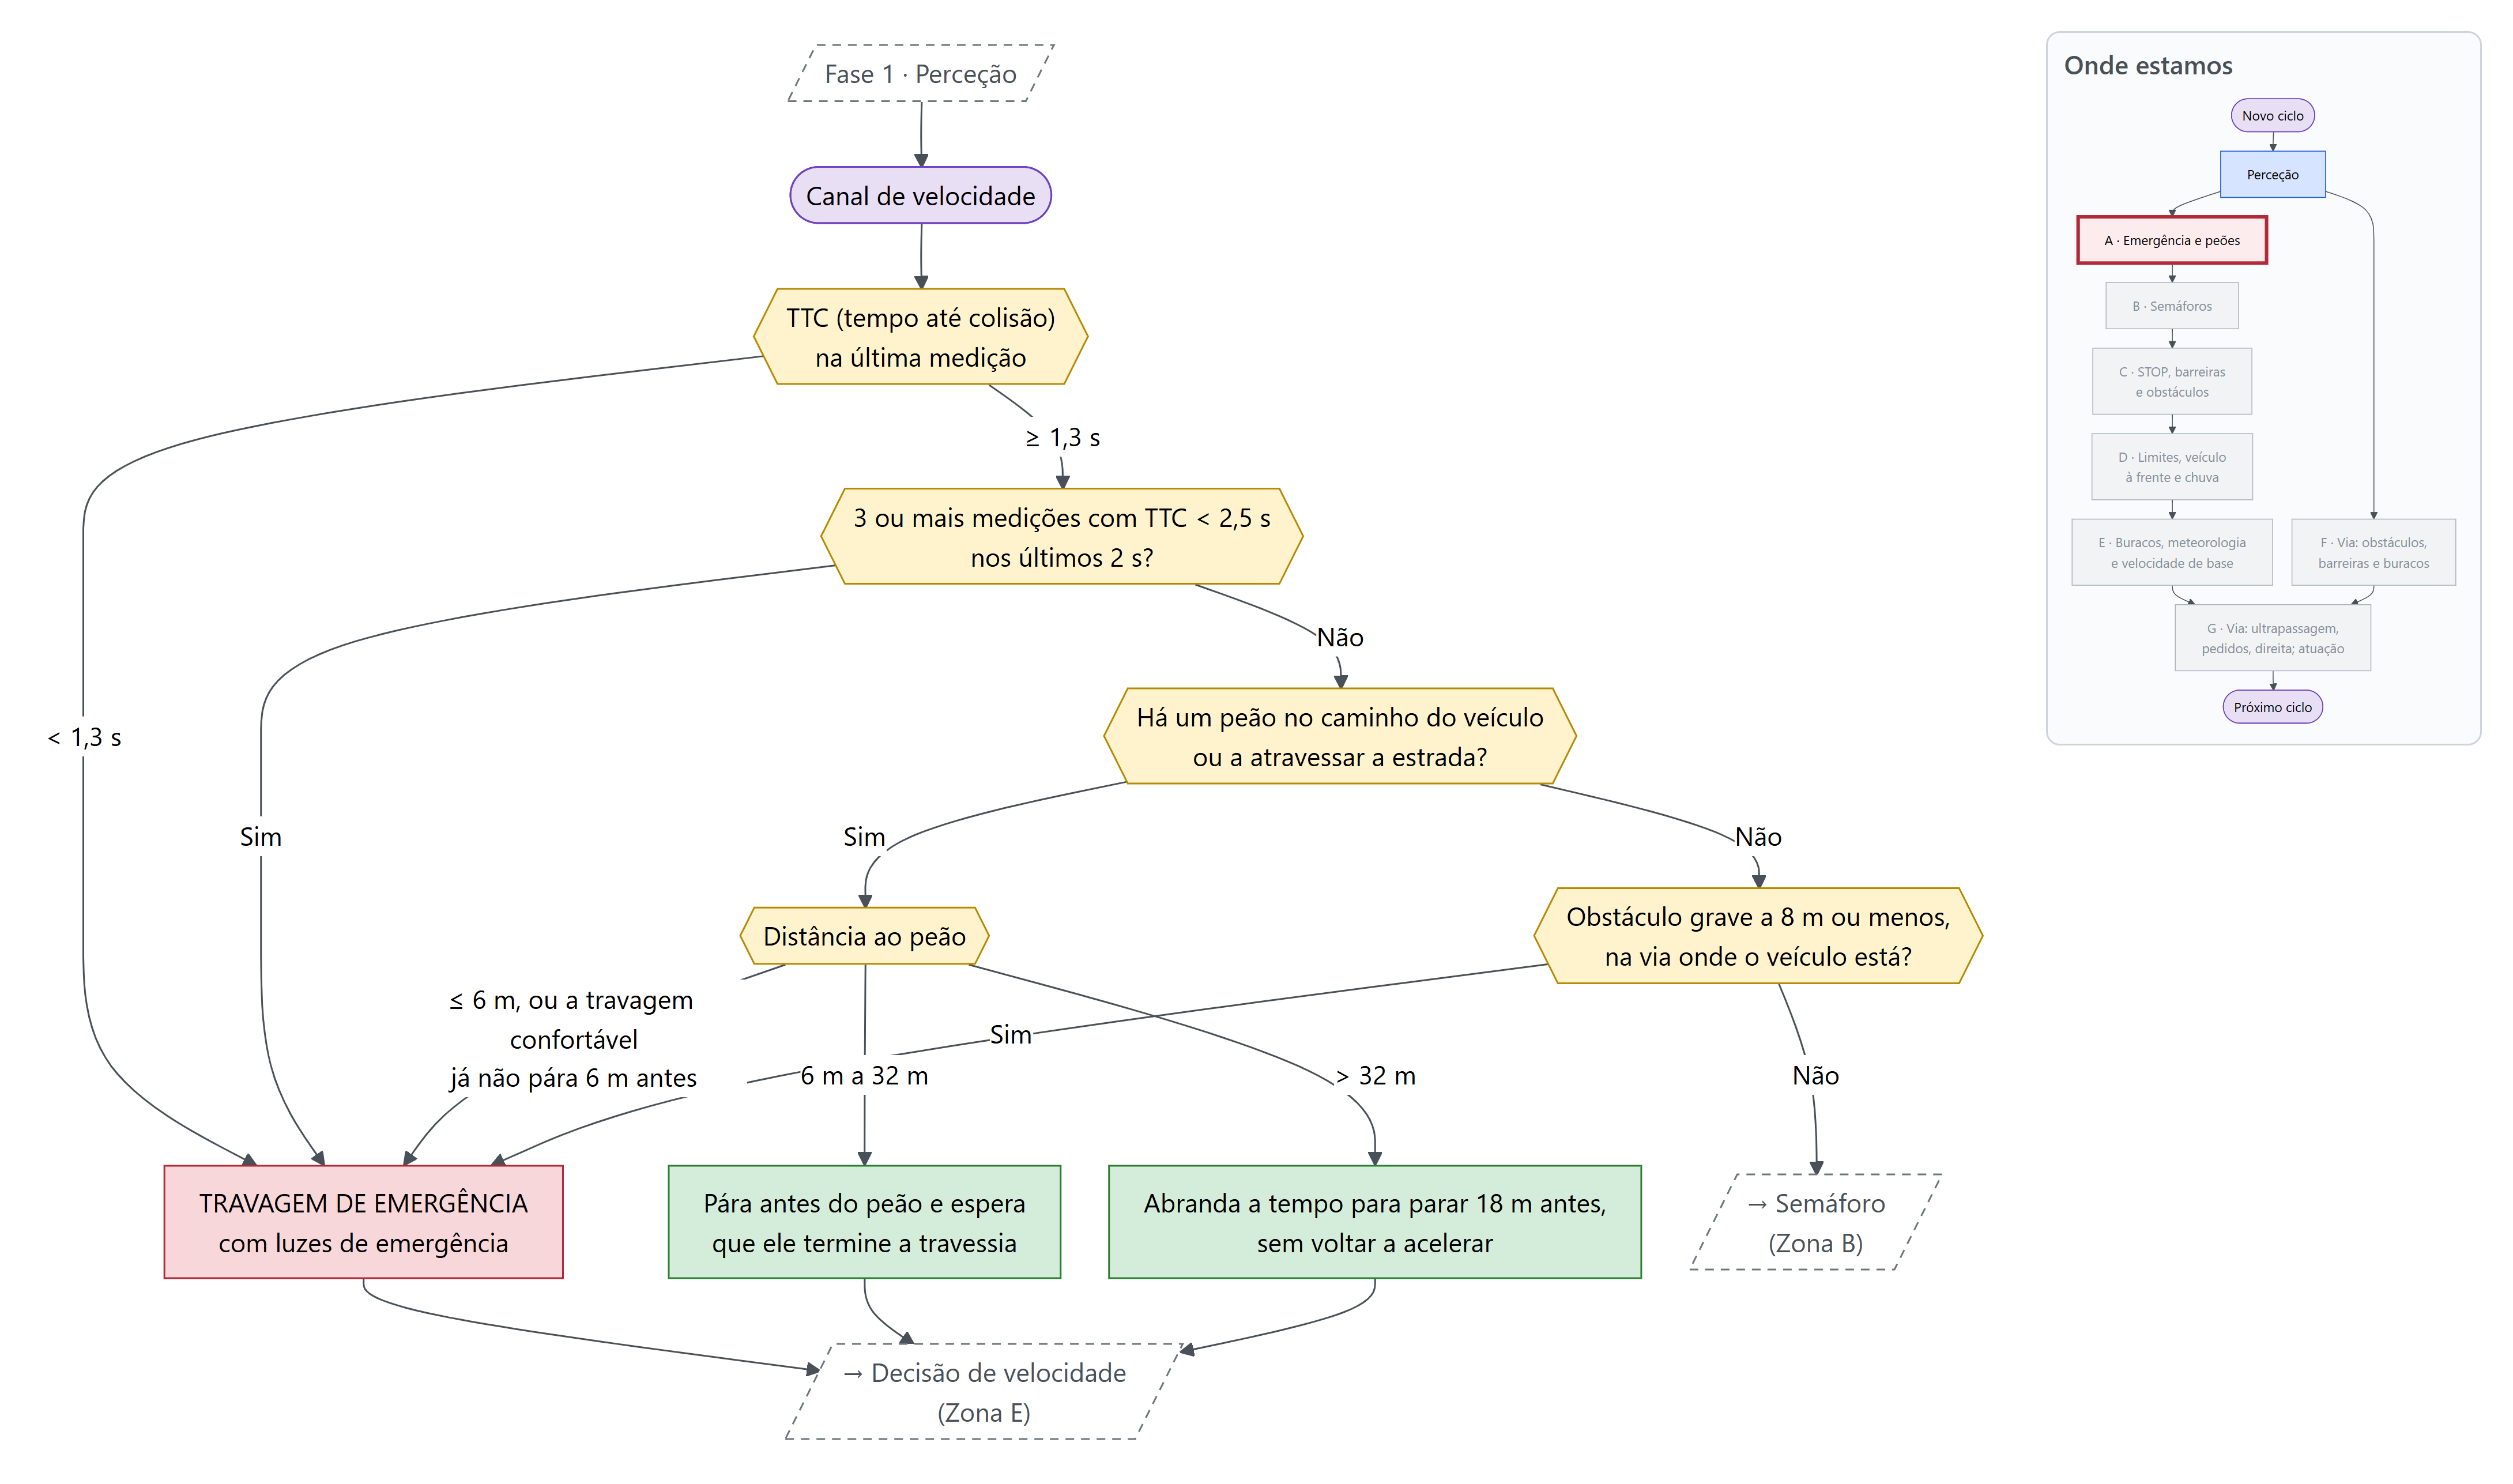
\includegraphics[width=\linewidth,height=0.80\textheight,keepaspectratio]{figuras/fig12_zona_a_emergencia_e_peoes}
\caption{Zona A: emergência e peões}\label{fig:12}
\end{figure}

\begin{landscape}
\begin{figure}[H]
\centering
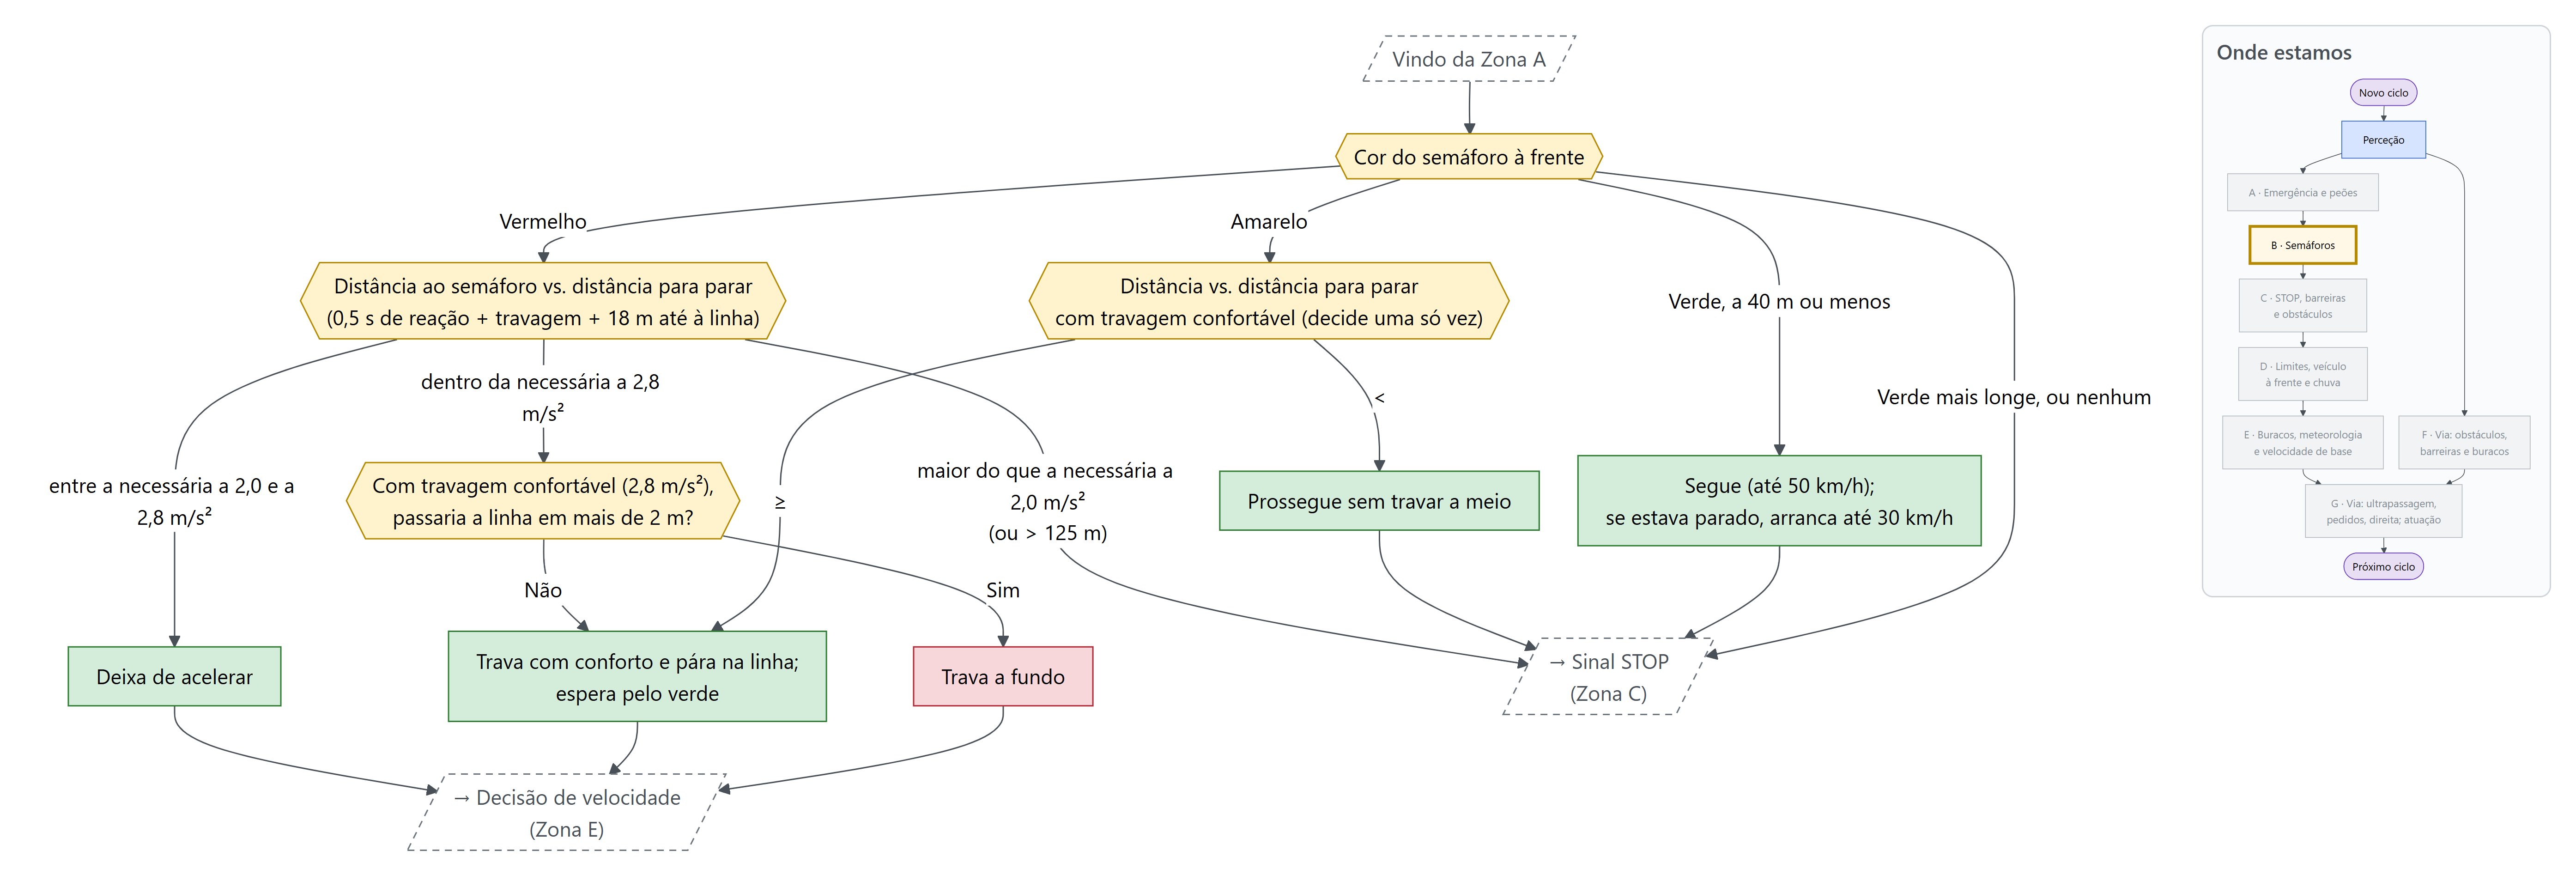
\includegraphics[width=\linewidth,height=0.82\textheight,keepaspectratio]{figuras/fig13_zona_b_semaforos}
\caption{Zona B: semáforos}\label{fig:13}
\end{figure}
\end{landscape}

\begin{landscape}
\begin{figure}[H]
\centering
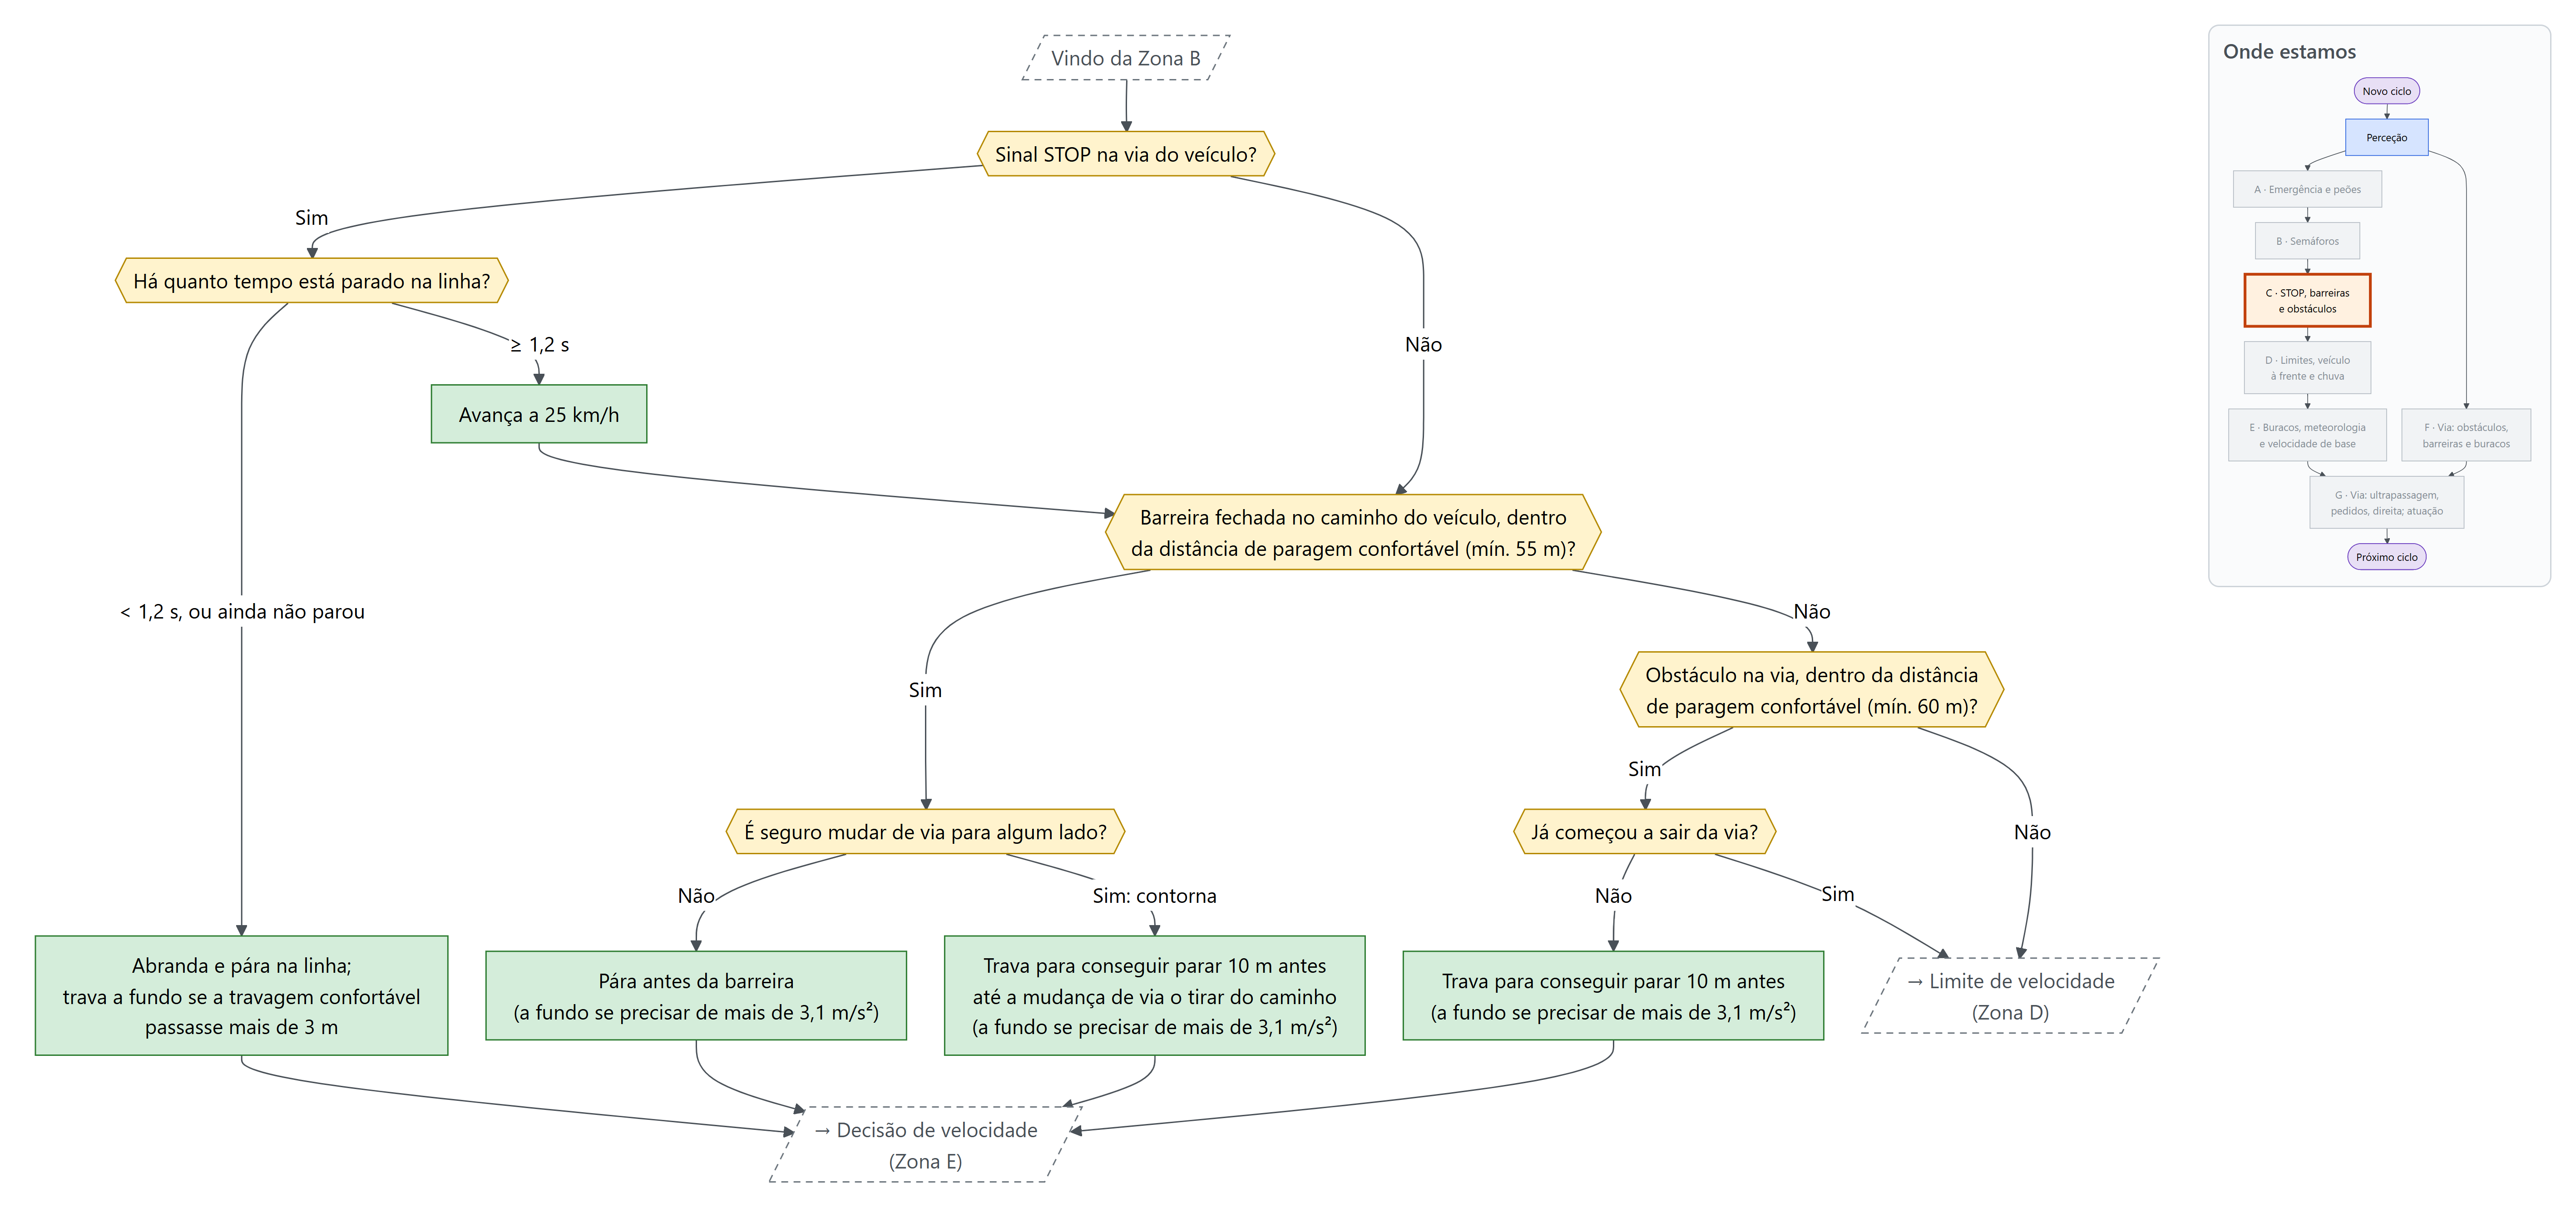
\includegraphics[width=\linewidth,height=0.82\textheight,keepaspectratio]{figuras/fig14_zona_c_stop_barreiras_e}
\caption{Zona C: STOP, barreiras e obstáculos}\label{fig:14}
\end{figure}
\end{landscape}

\begin{figure}[H]
\centering
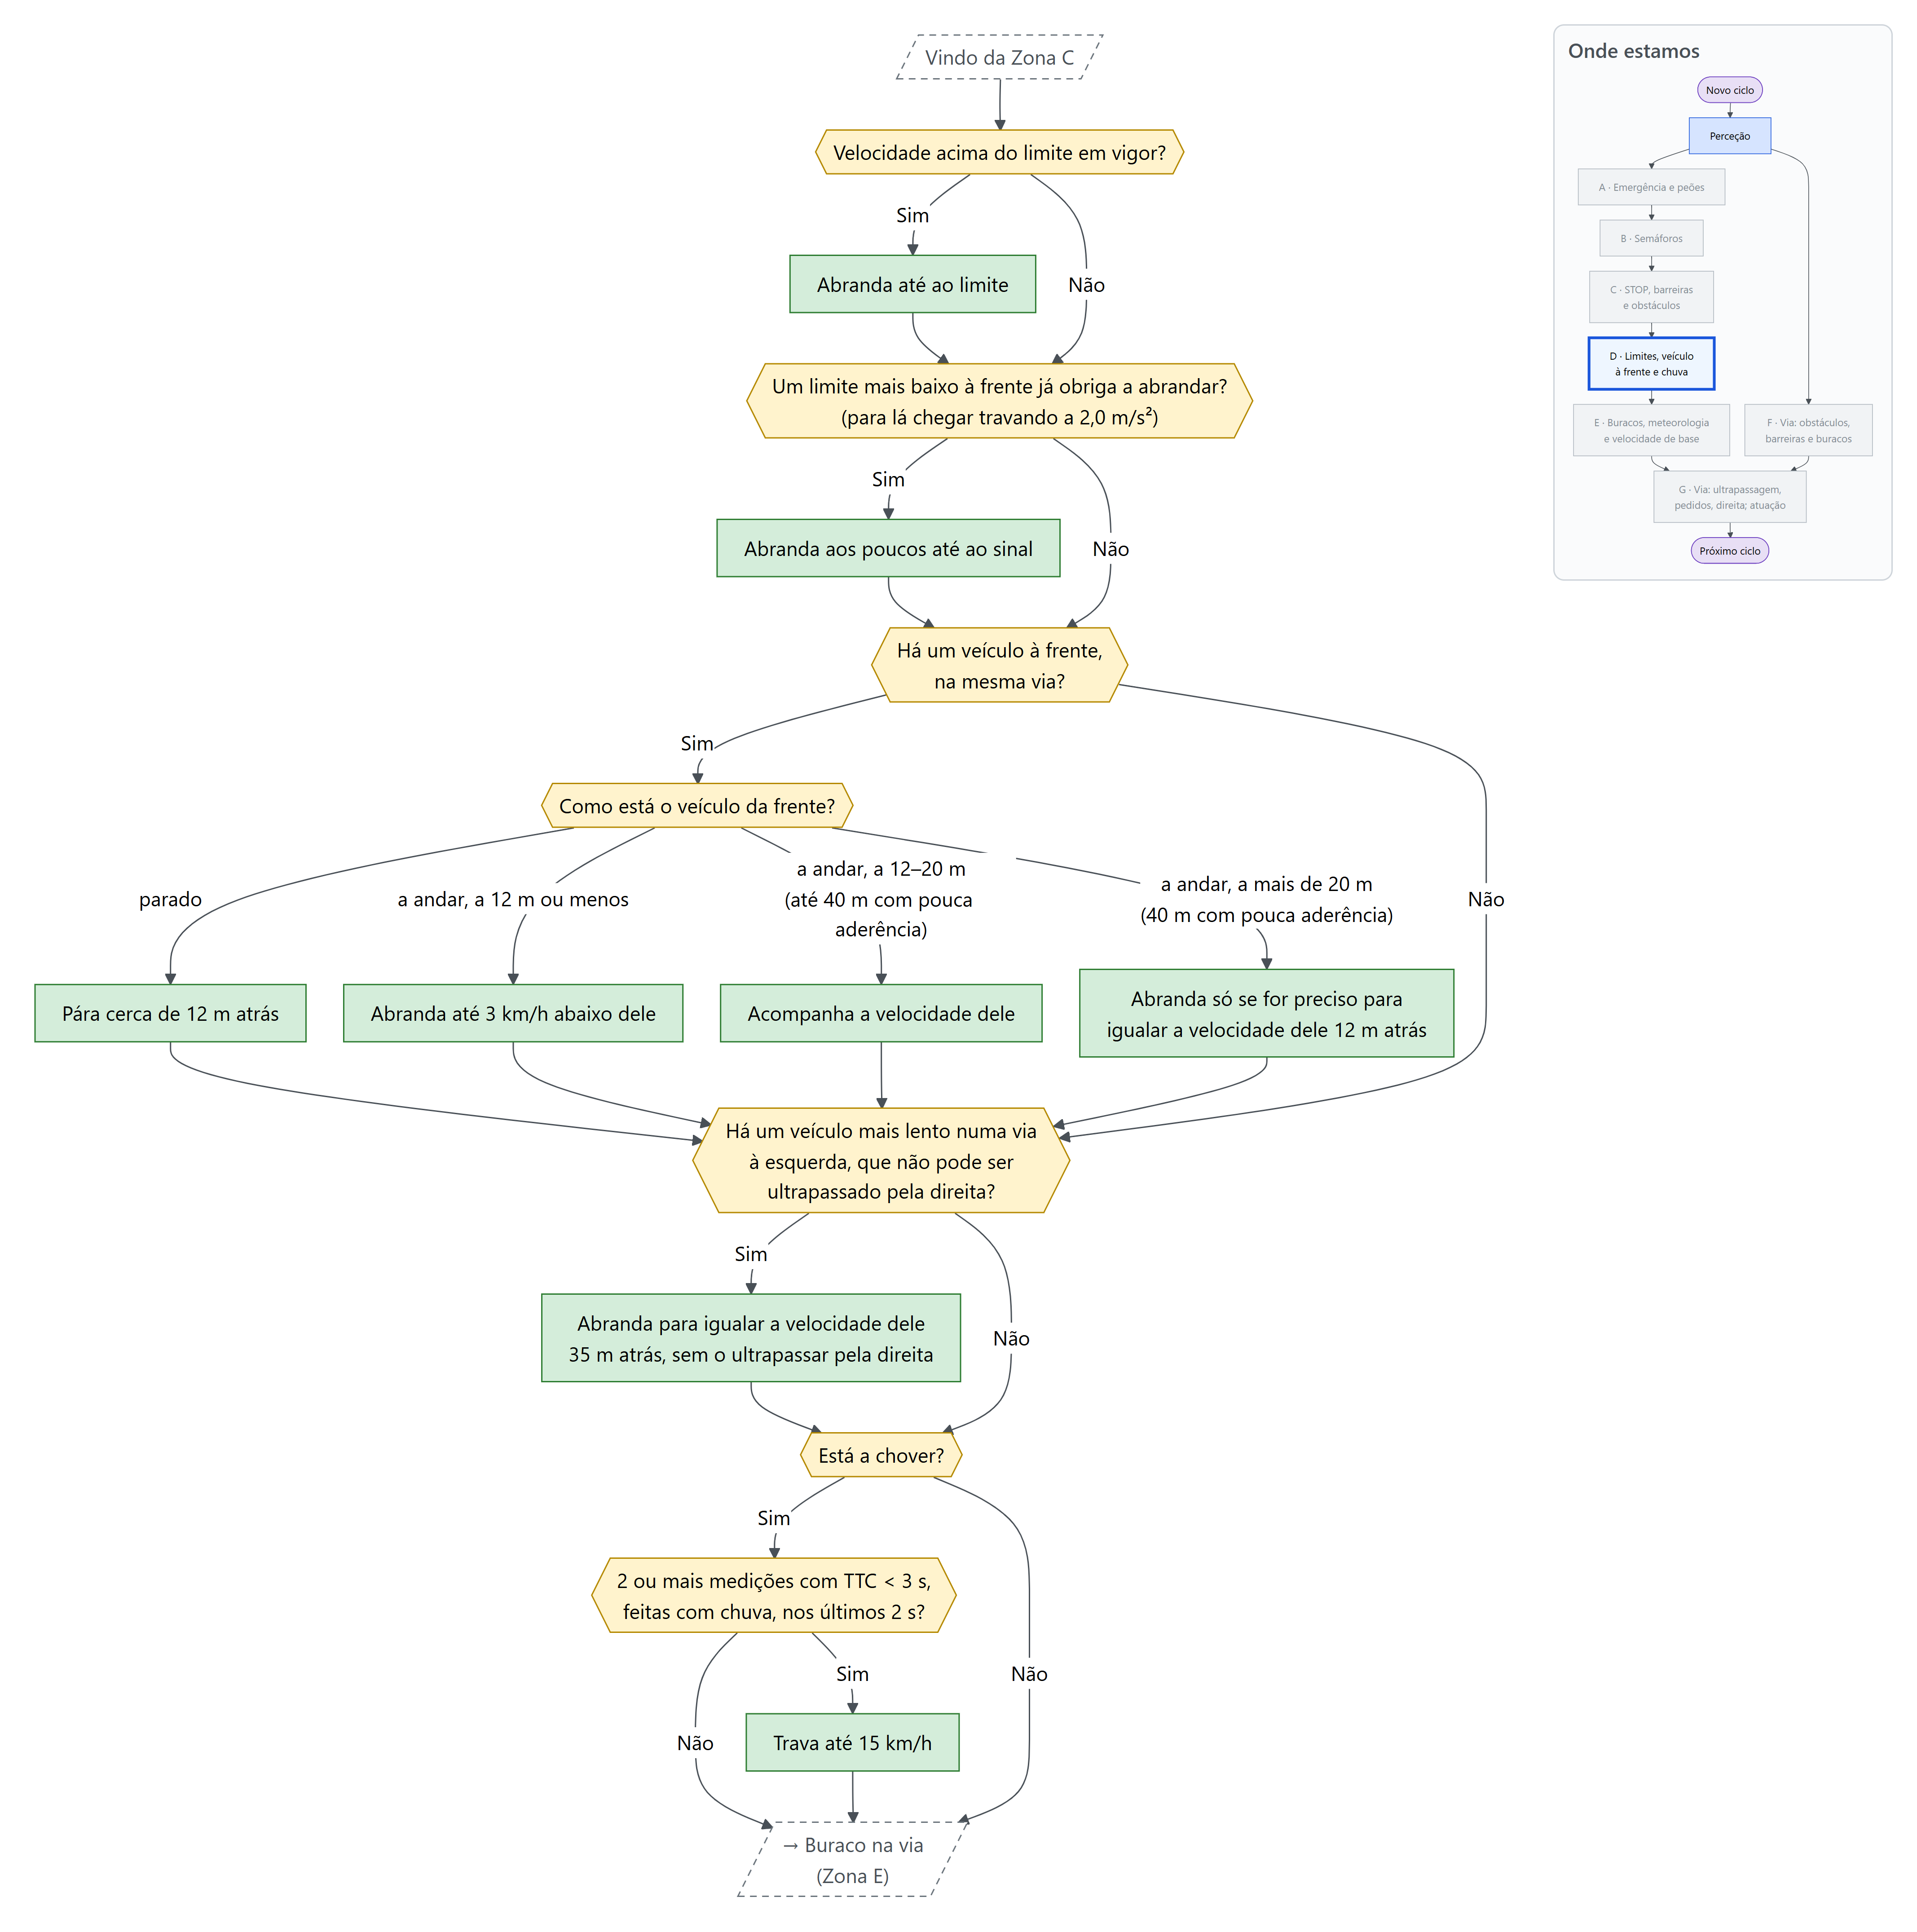
\includegraphics[width=\linewidth,height=0.80\textheight,keepaspectratio]{figuras/fig15_zona_d_limites_veiculo_a_frente}
\caption{Zona D: limites, veículo à frente e chuva}\label{fig:15}
\end{figure}

\begin{figure}[H]
\centering
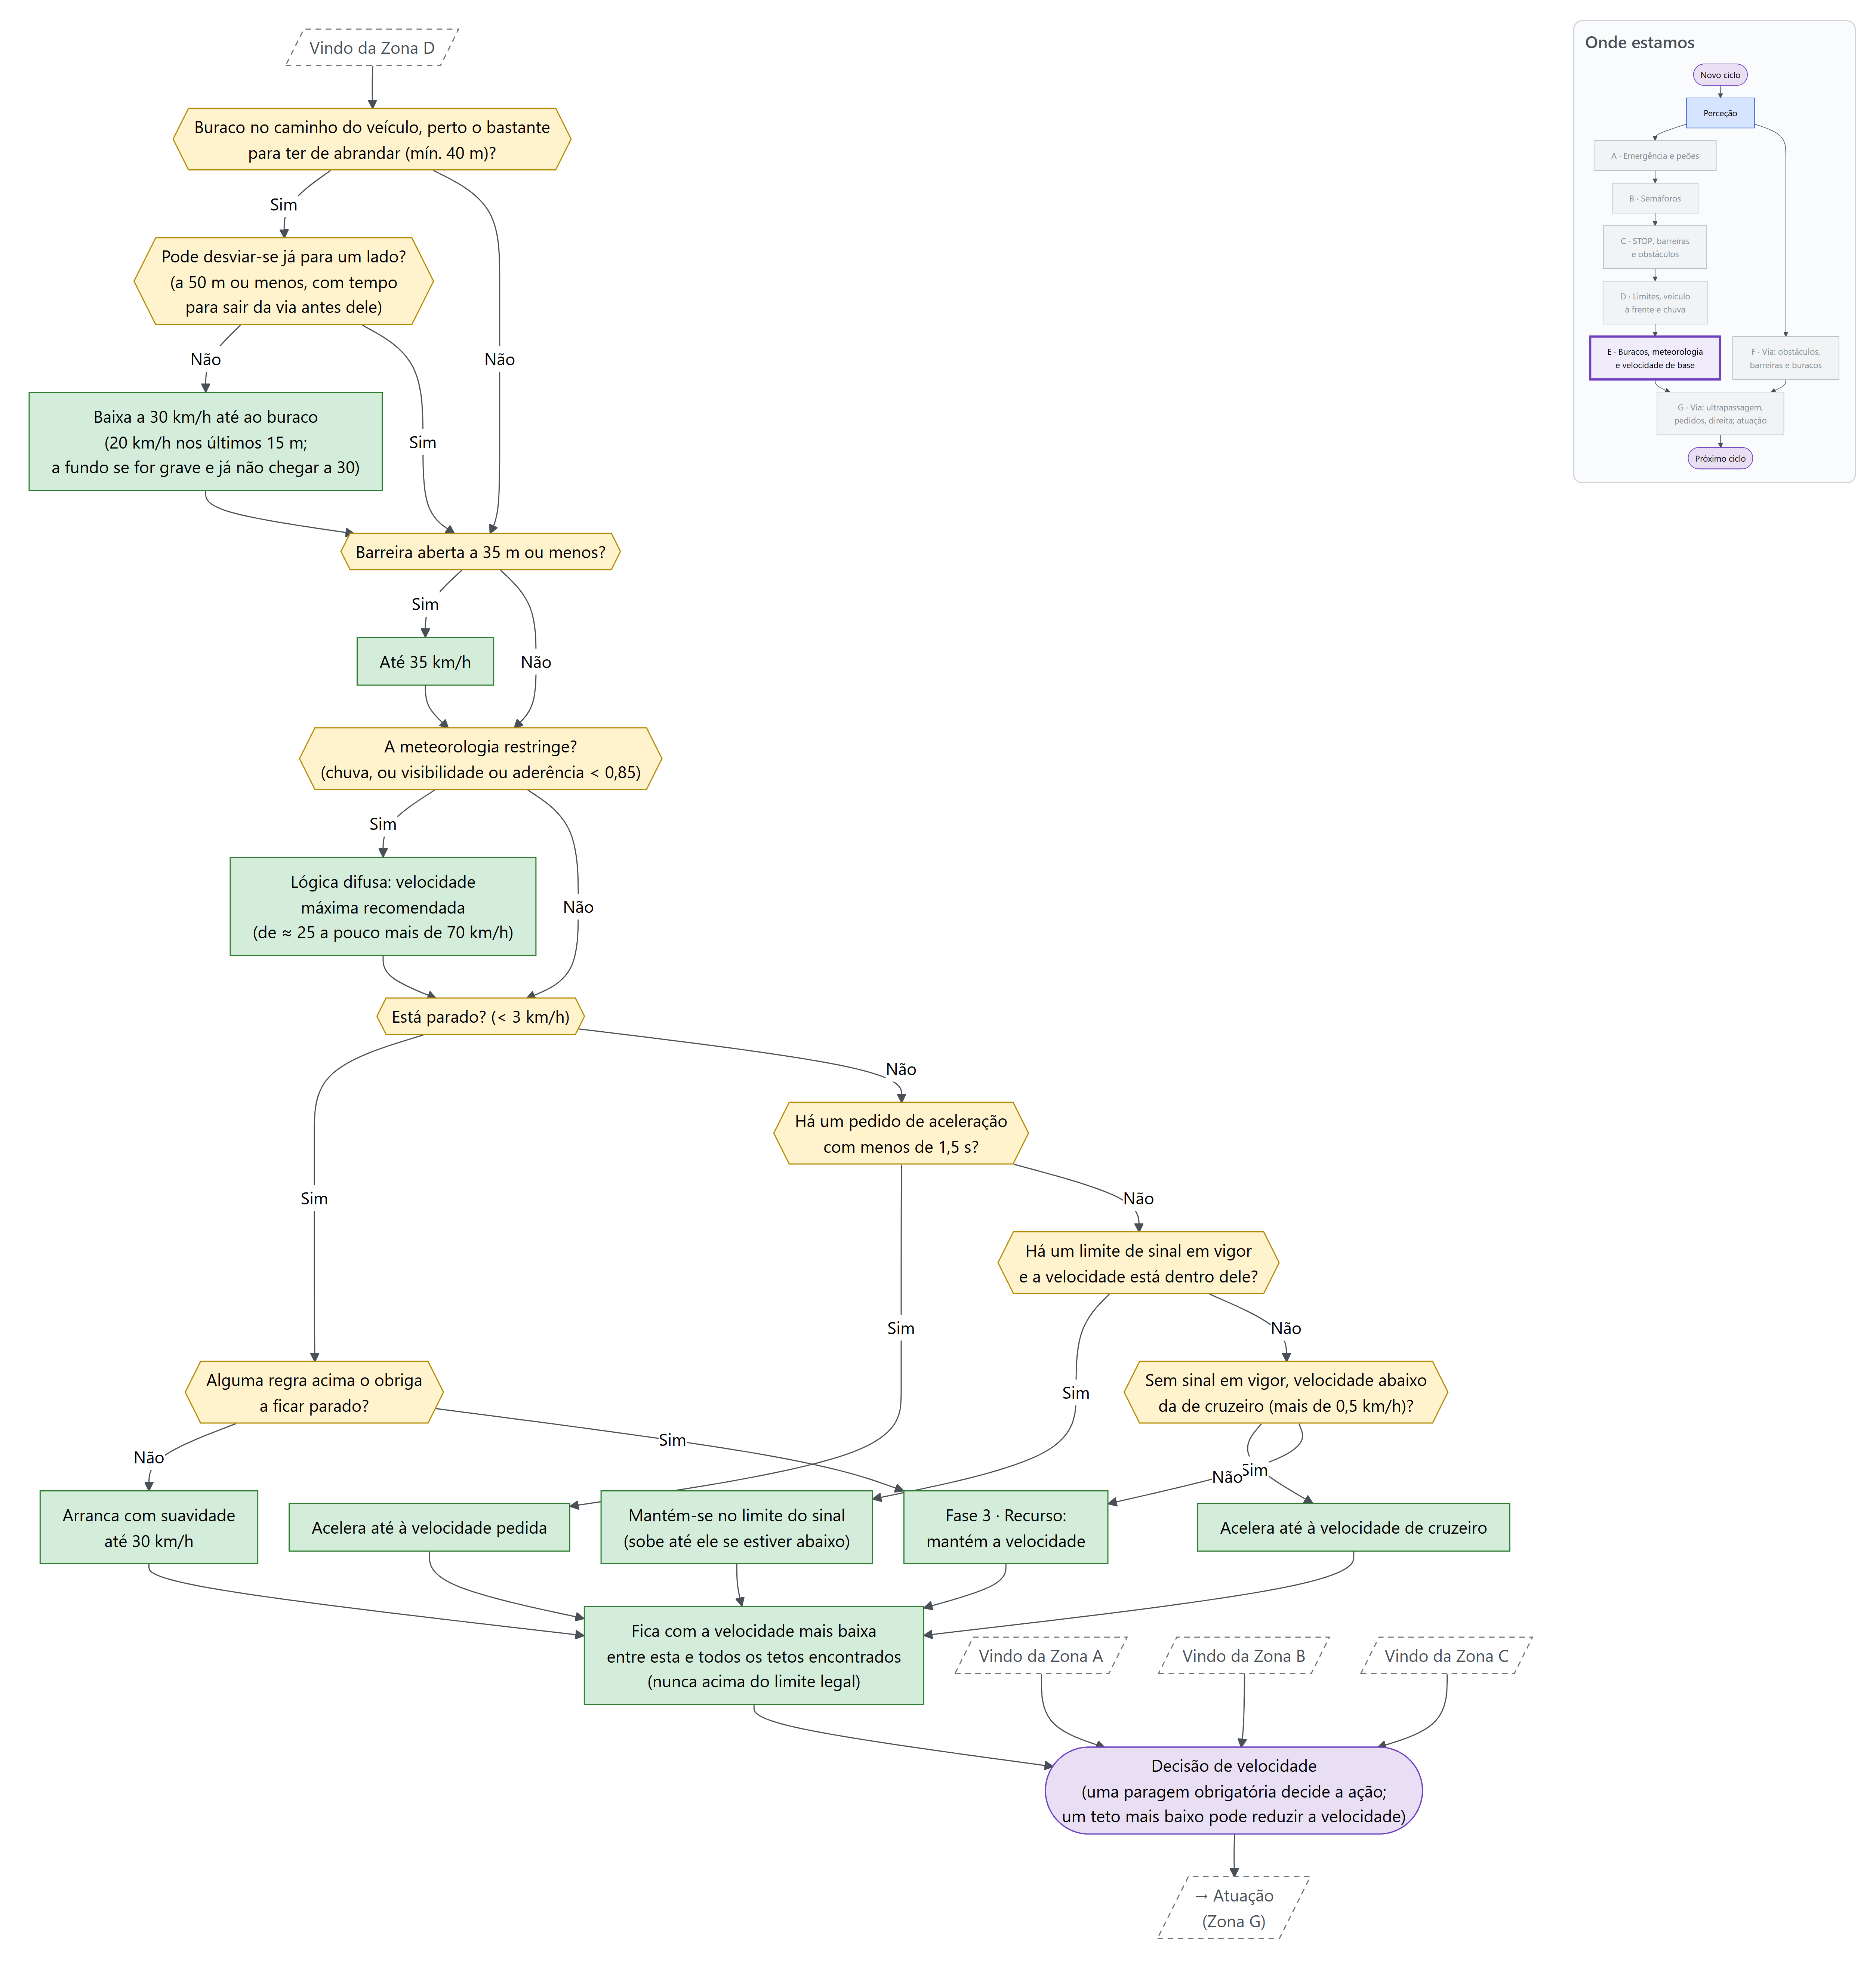
\includegraphics[width=\linewidth,height=0.80\textheight,keepaspectratio]{figuras/fig16_zona_e_buracos_meteorologia_e}
\caption{Zona E: buracos, meteorologia e velocidade de base}\label{fig:16}
\end{figure}

\begin{landscape}
\begin{figure}[H]
\centering
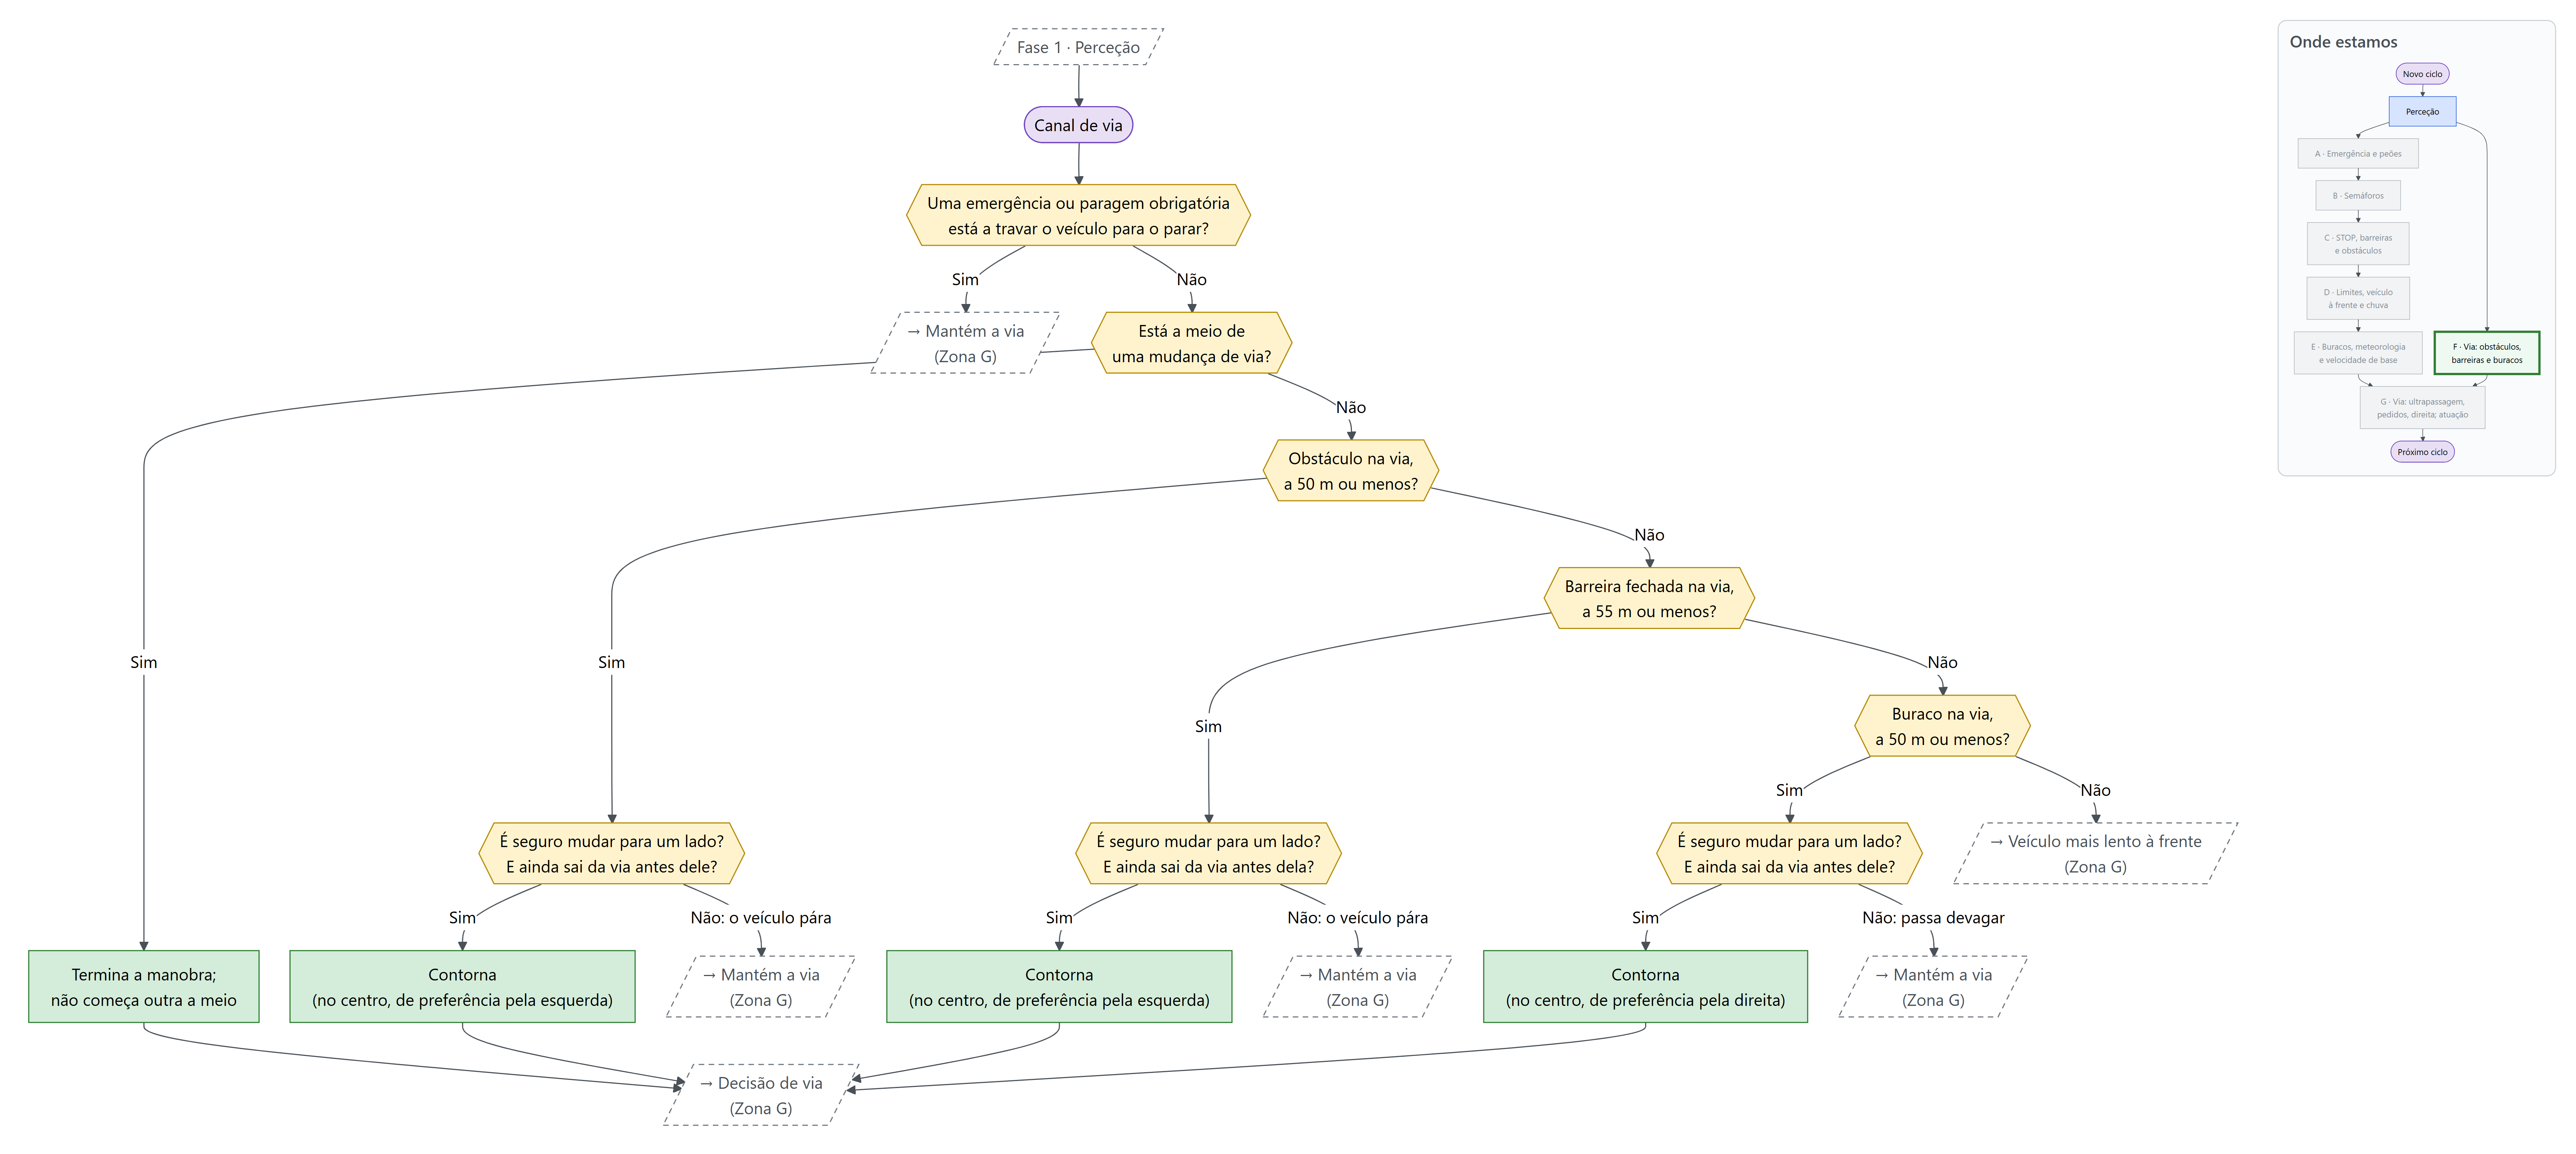
\includegraphics[width=\linewidth,height=0.82\textheight,keepaspectratio]{figuras/fig17_zona_f_canal_de_via_perante}
\caption{Zona F: canal de via perante obstáculos, barreiras e buracos}\label{fig:17}
\end{figure}
\end{landscape}

\begin{figure}[H]
\centering
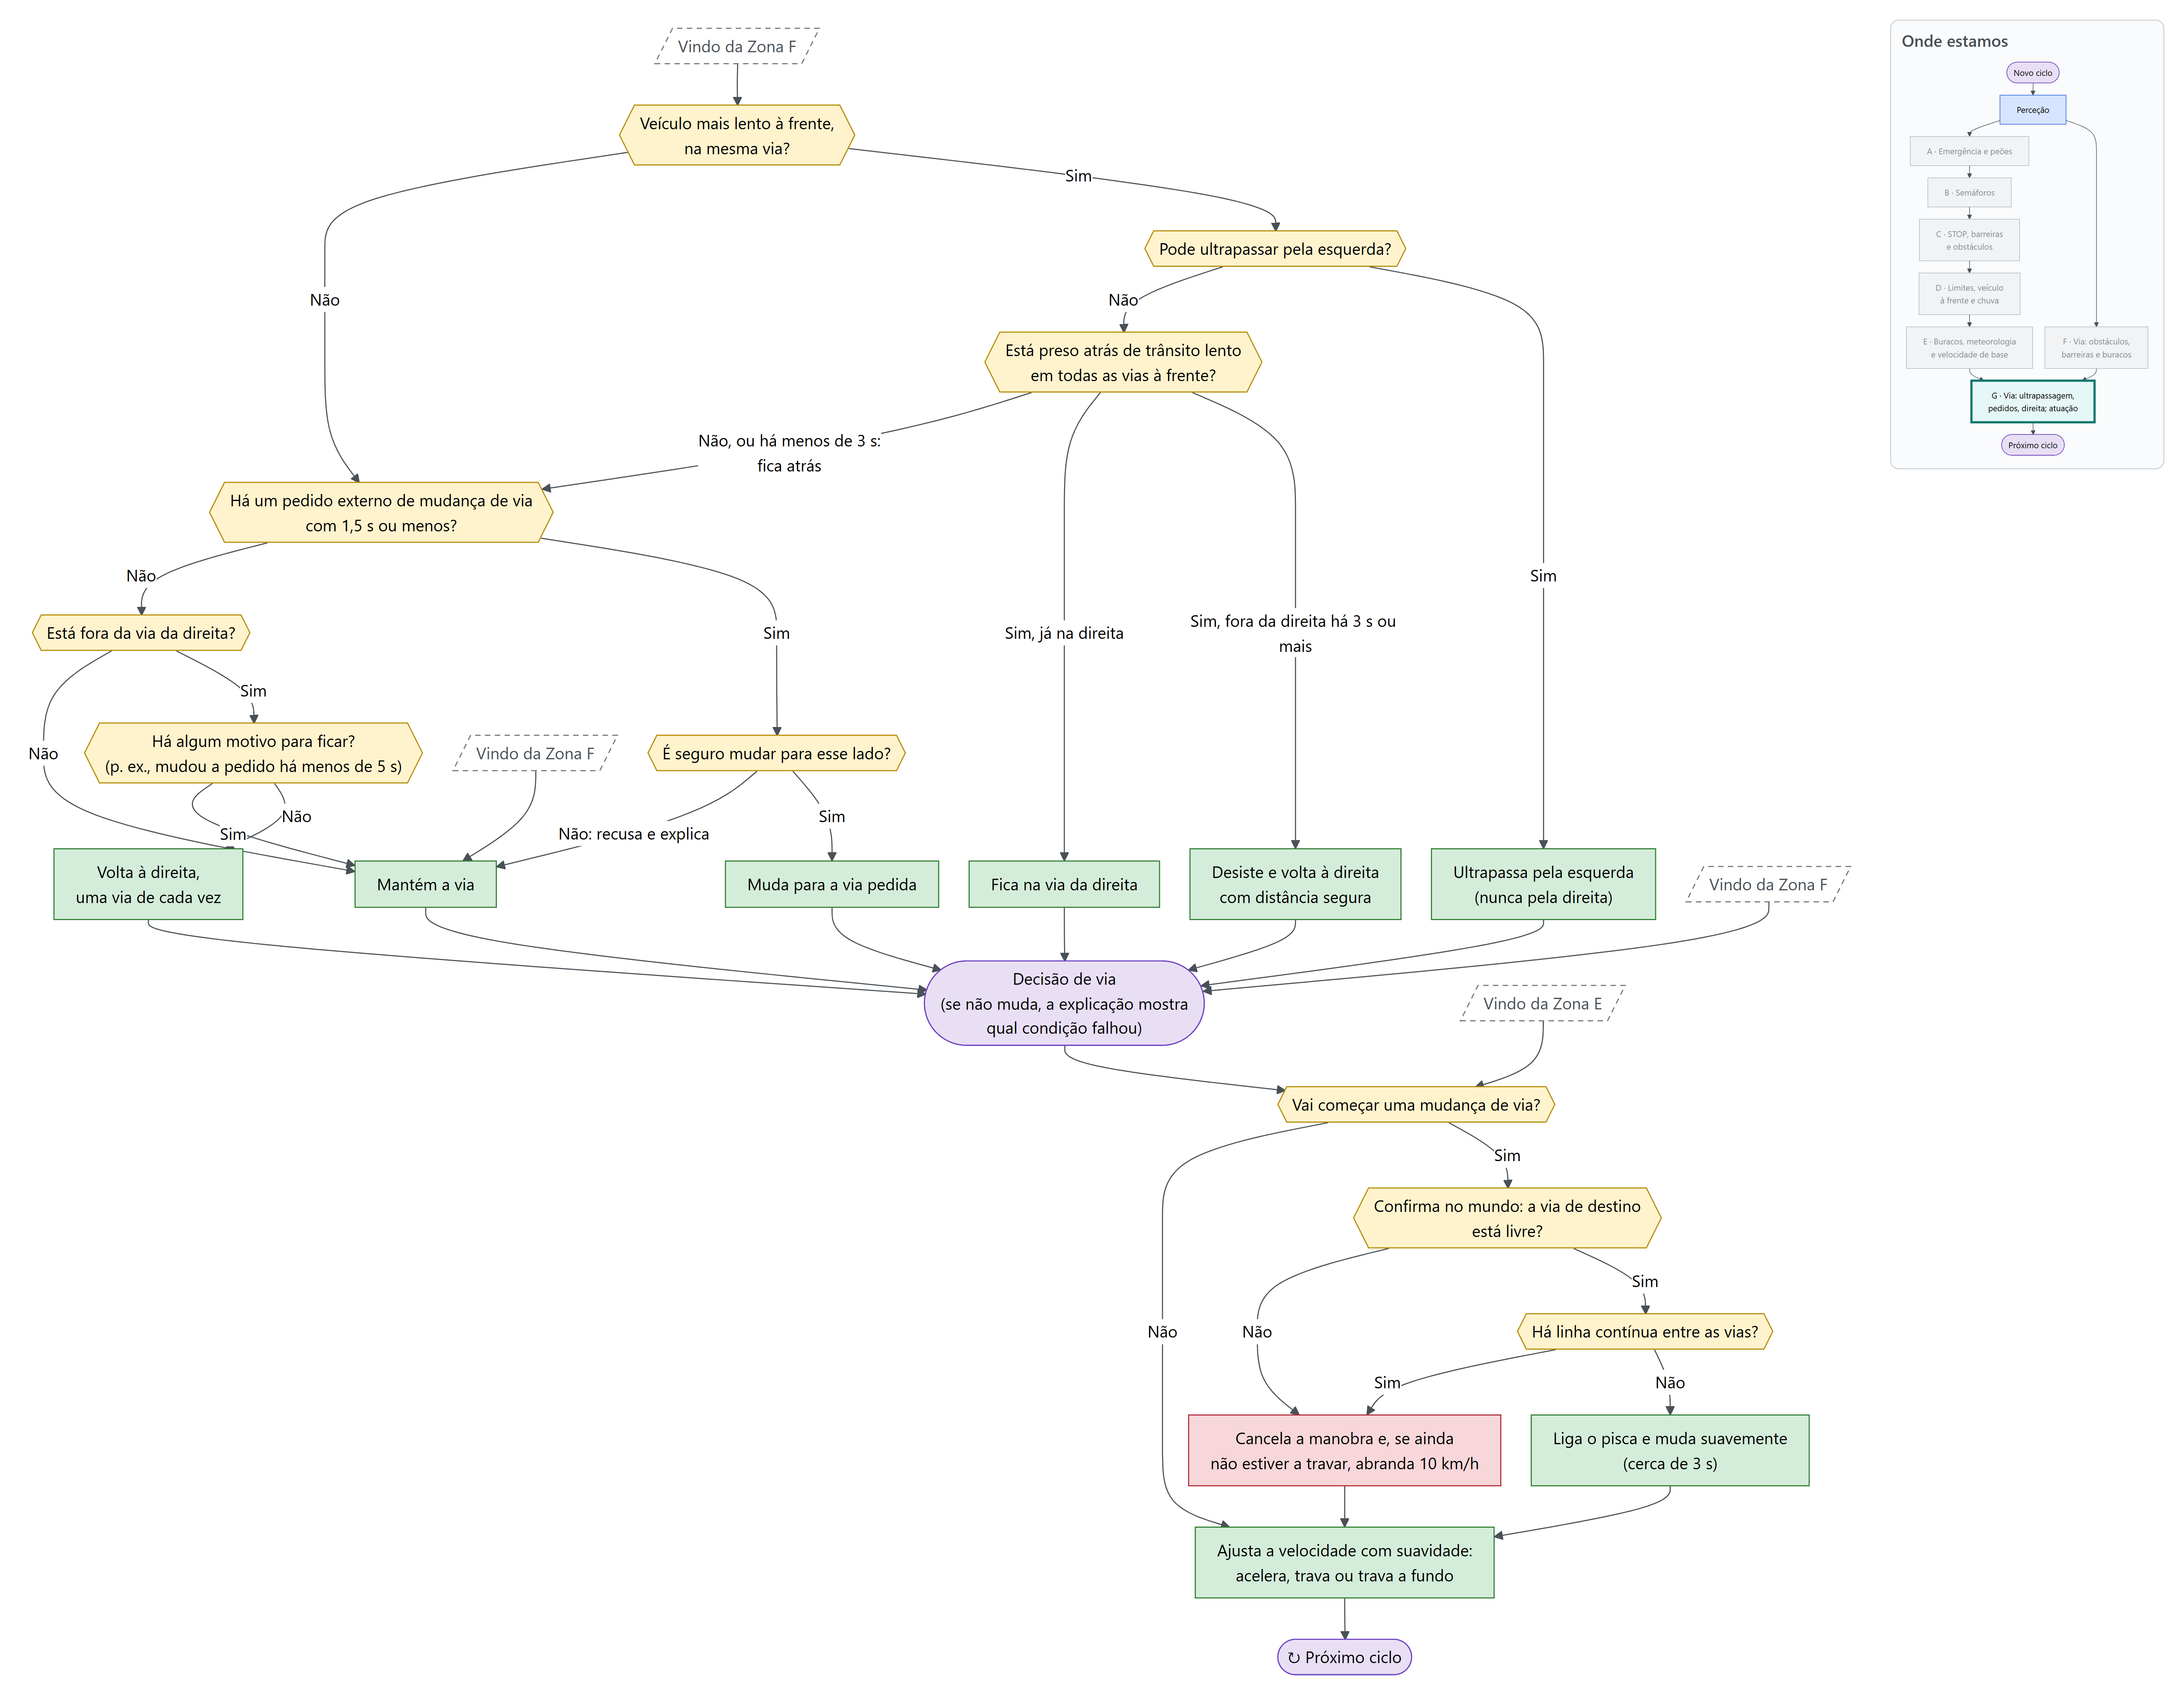
\includegraphics[width=0.90\linewidth,height=0.80\textheight,keepaspectratio]{figuras/fig18_zona_g_ultrapassagem_pedidos}
\caption{Zona G: ultrapassagem, pedidos, regresso à direita e atuação}\label{fig:18}
\end{figure}
